\documentclass[11pt]{article}
\usepackage[margin=1in]{geometry}
\usepackage{amsmath}
\usepackage{booktabs}
\usepackage{graphicx}
\usepackage{float}
\usepackage[hidelinks]{hyperref}
\emergencystretch=3em

\newcommand{\code}[1]{\texttt{#1}}

\title{Ring-down tests of the DTU10MW blade with and without the mount bolt}
\author{Ilan Upfal}
\date{29 October 2026, revised 12 November 2026}

\begin{document}
\maketitle

\section*{Summary}

On 21 October we flicked the blade tip and recorded the ring-down twice: first
with the mount bolt missing, then with it fitted. This note first gives the
bolted results (Section~\ref{sec:bolted}), then interprets them with the beam
model of the blade (Section~\ref{sec:interp}), then compares the bolted and
no-bolt blade (Section~\ref{sec:nobolt}), and finally asks which of the two
describes the production experiments of 6--15 October
(Section~\ref{sec:production}).

\paragraph{The bolted blade.}
\begin{enumerate}
  \item \textbf{Its low peaks are at 62, 117, 146 and 162\,Hz.} 62 and
        162\,Hz are flapwise and match the high-speed video; 117 and 146\,Hz
        are edgewise. Only the 117\,Hz peak moves the blade root much.
  \item \textbf{The 62\,Hz mode has a damping ratio of 1.31\%,} consistent
        across 30 flicks, and higher at large amplitude. The edgewise damping
        could not be measured reliably.
\end{enumerate}

\paragraph{Interpreted with the beam model.}
\begin{enumerate}
  \setcounter{enumi}{2}
  \item \textbf{The first edge mode is at 146\,Hz,} not 117\,Hz as we first
        read it. With 146\,Hz, the measured frequency ratios are both about
        10\% below the clamped beam model's (edge/flap 2.35 against 2.60,
        second/first flap 2.61 against 2.97); with 117\,Hz the edge ratio would
        be 27\% low, out of line with the flap ratio.
  \item \textbf{The 117\,Hz peak is most likely a mount mode.} The clamped
        model has no mode there, the peak moves the root, and it is the one
        the bolt changes most. This is our reading of the data, not yet a
        measurement of the mount.
\end{enumerate}

\paragraph{With and without the bolt.}
\begin{enumerate}
  \setcounter{enumi}{4}
  \item \textbf{Every low peak is lower.} The first flap mode drops from 62
        to 55\,Hz ($-11\%$) and the mount mode from 117 to 85\,Hz
        ($-27\%$). The first edge and second flap modes (146 and 162\,Hz)
        become a close pair at 131 and 138\,Hz; which is which cannot be told
        from these data. Higher modes move by 5\% or less.
  \item \textbf{The first flap mode is more damped:} 2.16\% against 1.31\%,
        with a stronger dependence on amplitude.
\end{enumerate}

\paragraph{The experiments.}
\begin{enumerate}
  \setcounter{enumi}{6}
  \item \textbf{The production runs match the no-bolt blade.} In the slowest
        runs, at the angles where the blade barely vibrates, the spectra peak
        at 84--86 and 131--133\,Hz on every test day with such a run (6, 9 and
        14 October). There is nothing at the bolted 117, 146 or 162\,Hz. The
        bolt was most likely missing for the whole campaign, and the no-bolt
        frequencies are the ones to compare the experiments with.
  \item \textbf{The 85\,Hz peak in the experiments is then the loose mount,}
        not a blade mode. That the largest low-speed response is the mount
        rocking is itself worth knowing.
  \item \textbf{In the tunnel the 131\,Hz peak moves mostly edgewise.} In the
        ring-down it is strongest flapwise. With two modes at 131 and
        138\,Hz, the tunnel may be exciting the edgewise one of the pair.
        Either way it is best referred to by frequency.
  \item \textbf{At high speed the blade responds at neither configuration's
        frequencies.} At 6.9\,m/s the 85 and 131\,Hz peaks give way to a
        single peak at 109--111\,Hz. The ring-down frequencies describe the
        blade at low speed only.
\end{enumerate}

\section{The tests}

Both runs used the experiment mount at the experiment settings (mounting
angle $84.1^\circ$, sweep $-30^\circ$), in still air. The blade tip was
flicked by hand, either flapwise or edgewise, and each flick was recorded for
10\,s with all four accelerometers. One 10\,s capture with no flick gives the
noise floor.

\begin{center}
\begin{tabular}{lccc}
  \toprule
  Run & Time (21 Oct) & Flap flicks & Edge flicks \\
  \midrule
  \code{DTU10MW\_rigid4k\_ringdown\_NOBOLT} & 14:19--14:55 & 31 & 30 \\
  \code{DTU10MW\_rigid4k\_ringdown}         & 15:09--15:35 & 30 & 30 \\
  \bottomrule
\end{tabular}
\end{center}

This note uses sensor~4, nearest the tip, which moves the most. Its $y$ axis
is edgewise and its $z$ axis flapwise: flap flicks ring mostly in $z$ and
edge flicks mostly in $y$. The $x$ axis is spanwise and barely moves.

\paragraph{Spectra.} The spectra are made as in
\code{plot\_ringdown\_psd.py}. Each sample is placed on the sensor's actual
1493\,Hz sample grid, and the samples our read loop drops are left as gaps
(\code{reports/accel\_sampling}, \code{reports/pcb\_manual\_notes}). Each
flick gives a Welch PSD from the onset of the ring-down (segments of 2048,
0.73\,Hz resolution), and the median over all flicks of one kind is shown.
The gaps make weak copies of every peak at $\pm14.9$\,Hz. With 84 samples
kept out of every 100, each copy carries about 3\% of its parent's PSD; we
measure 2--5\% on the isolated 62\,Hz mode. A peak is therefore treated as a
copy, and not counted as a mode, only if it sits at a copy position of a
stronger peak \emph{and} is below 20\% of it. (An earlier version of this
note used the position alone and so discarded the bolted 146\,Hz mode.)
Frequencies above
about 150\,Hz are uncertain by up to one copy spacing (15\,Hz), because they
depend on the exact sample rate.

\paragraph{Damping.} The usual ways to measure damping from a ring-down
(log decrement from successive peaks, or a band-pass filter and envelope)
assume a continuous signal. Here every 84 consecutive samples are followed by
a gap of about 16 lost samples, which would bias them. The spectral
half-power width does not work either: at $\sim$1\% damping the 62\,Hz peak is
only $\sim$1.2\,Hz wide, close to the 0.73\,Hz resolution. We therefore use
the reads themselves (\code{ringdown\_damping.py}):
\begin{enumerate}
  \item Within each read (84 samples, 56\,ms), fit the signal by least
        squares, at the samples' true times on the 1493\,Hz grid, with a
        constant plus a sine and cosine at the mode frequency and at the two
        other strongest peaks of that channel. Fitting the neighbours together
        keeps them out of the mode's amplitude, even when a neighbour is only
        30\,Hz away (as in the no-bolt run). This gives the mode's amplitude
        $A$ in each read, unaffected by the gaps between reads.
  \item Keep the reads from the largest amplitude onward, skip any read in
        which the sensor clipped, and stop when $A$ falls below five times the
        noise floor (the same fit on the at-rest capture).
  \item Fit a straight line to $\ln A$ against time. For a decay
        $A \propto e^{-\zeta\omega t}$ its slope is $-\zeta\omega$, which
        gives the damping ratio $\zeta$.
\end{enumerate}
Each flick is fitted separately, so the spread over the 30 flicks of each
kind gives the uncertainty.

To check the method we built decaying sines with a known damping ratio, added
two neighbouring modes and noise, sampled them with the exact read and gap
timing of a real capture, and applied the method. It recovered
$\zeta = 0.50$, 1.30 and 2.00\% as 0.50, 1.29 and 1.99\% (median of 20
realizations each, all within 4\%), so the gaps and the neighbouring modes do
not bias it.

\section{The bolted blade: results}
\label{sec:bolted}

This section gives what the bolted ring-down measured. What the peaks are is
the subject of Section~\ref{sec:interp}.

\subsection{Peaks}

\begin{figure}[H]
  \centering
  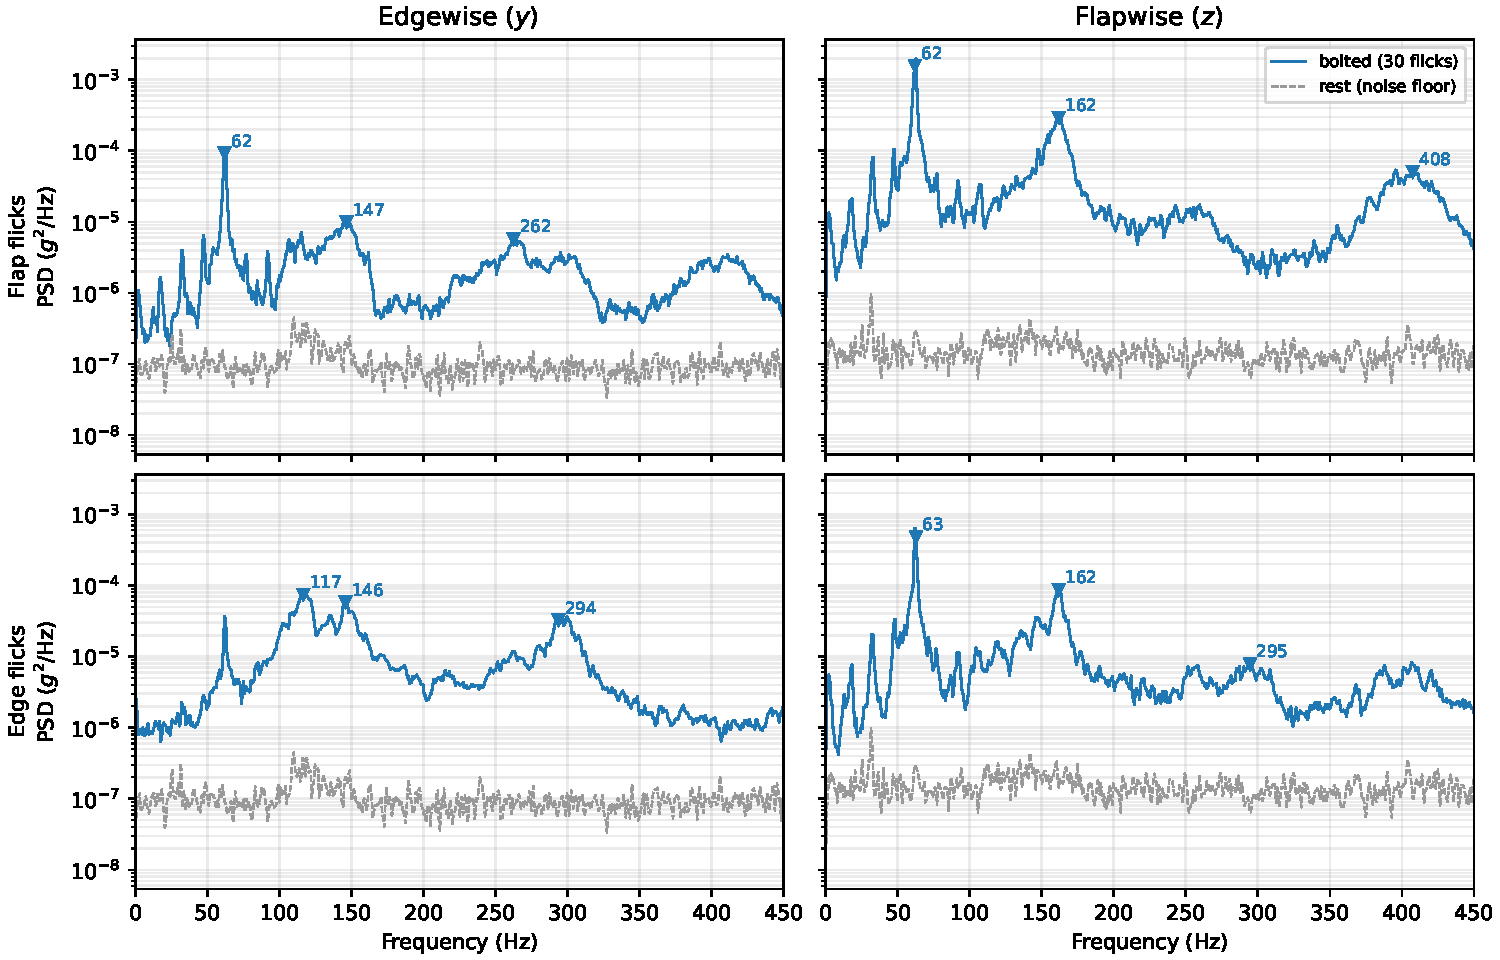
\includegraphics[width=\textwidth]{figs/ringdown_bolted.pdf}
  \caption{Bolted blade: median PSD of sensor~4. Rows: flap flicks, edge
  flicks. Columns: edgewise ($y$) and flapwise ($z$) axes. Triangles mark the
  three largest peaks after the batch-gap copies are removed. Grey: no-flick
  capture.}
  \label{fig:bolted}
\end{figure}

Figure~\ref{fig:bolted} shows the spectra and Table~\ref{tab:bolted} the
peaks. A peak's direction is the axis it is largest in and the flick that
rings it hardest.

\begin{table}[H]
  \centering
  \begin{tabular}{cll}
    \toprule
    Frequency (Hz) & Main axis & Rung hardest by \\
    \midrule
    62  & $z$ (flapwise) & flap flicks \\
    117 & $y$ (edgewise) & edge flicks \\
    146 & $y$, also strong in $z$ & edge flicks ($y$), flap flicks ($z$) \\
    162 & $z$ & flap flicks \\
    294 & $y$ & edge flicks \\
    408 & $z$ & flap flicks \\
    536 & $y$ & edge flicks \\
    \bottomrule
  \end{tabular}
  \caption{Peaks of the bolted blade, sensor~4. There is also a weak
  flapwise peak at 259\,Hz. The three highest are uncertain by about
  15\,Hz.}
  \label{tab:bolted}
\end{table}

\paragraph{Two edgewise peaks, at 117 and 146\,Hz.} Edge flicks ring two
edgewise peaks of similar size (Figure~\ref{fig:bolted}, lower left). The
146\,Hz peak sits 1\,Hz from a copy position of both the 117 and the
162\,Hz peak, but it is far too strong to be a copy: 75\% of the 117\,Hz
peak in $y$ and 37\% of the 162\,Hz peak in $z$, against the 2--5\% a copy
carries. In the flap flicks it is the largest edgewise peak between 95 and
185\,Hz. It is rung hard in $z$ by flap flicks as well.

\paragraph{The flicks are not pure.} An edge flick also rings the 62\,Hz
peak, and in $z$ that peak is about eight times stronger than the 117\,Hz
peak is in $y$. The directions in Table~\ref{tab:bolted} are where each peak
is largest, not the only place it appears.

\paragraph{Agreement with the high-speed video.} The video of a flapwise
ring-down gave 62.7 and 164.5\,Hz (\code{reports/accel\_sampling},
\code{reports/pcb\_manual\_notes}), matching the 62 and 162\,Hz peaks.

\subsection{Motion along the span}

\begin{figure}[H]
  \centering
  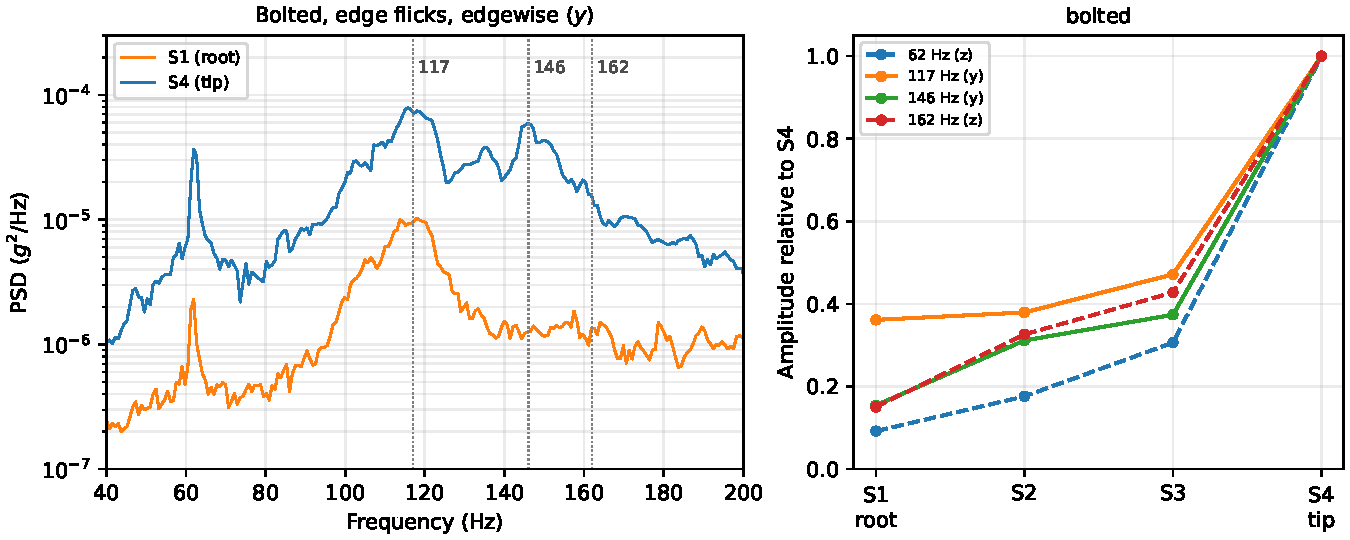
\includegraphics[width=0.85\textwidth]{figs/root_motion.pdf}
  \caption{Bolted blade, motion at the root. Left: edge flicks, edgewise PSD
  at sensor~1 (root) and sensor~4 (tip). Right: amplitude
  ($\sqrt{\mathrm{PSD}}$) of each peak along the span, relative to the tip,
  in the flick and axis that ring it hardest. The sensors' exact spanwise
  positions are not used; they are plotted in order.}
  \label{fig:root}
\end{figure}

The four sensors run from the root (S1) to the tip (S4). Figure~\ref{fig:root}
shows how much each peak moves the root:
\begin{itemize}
  \item At sensor~1 the edge flicks show a single edgewise peak, at 117\,Hz,
        100 times the noise floor and 7 times the surrounding spectrum. The
        146 and 162\,Hz peaks do not rise above the surrounding spectrum there
        (left).
  \item Sensor~1 moves 36\% as much as the tip at 117\,Hz, against 15\% at
        146 and 162\,Hz and 9\% at 62\,Hz (right). In $z$ the three inner
        sensors move almost together at 117\,Hz (0.53, 0.53, 0.58 of the
        tip).
\end{itemize}

\subsection{Damping}

\begin{figure}[H]
  \centering
  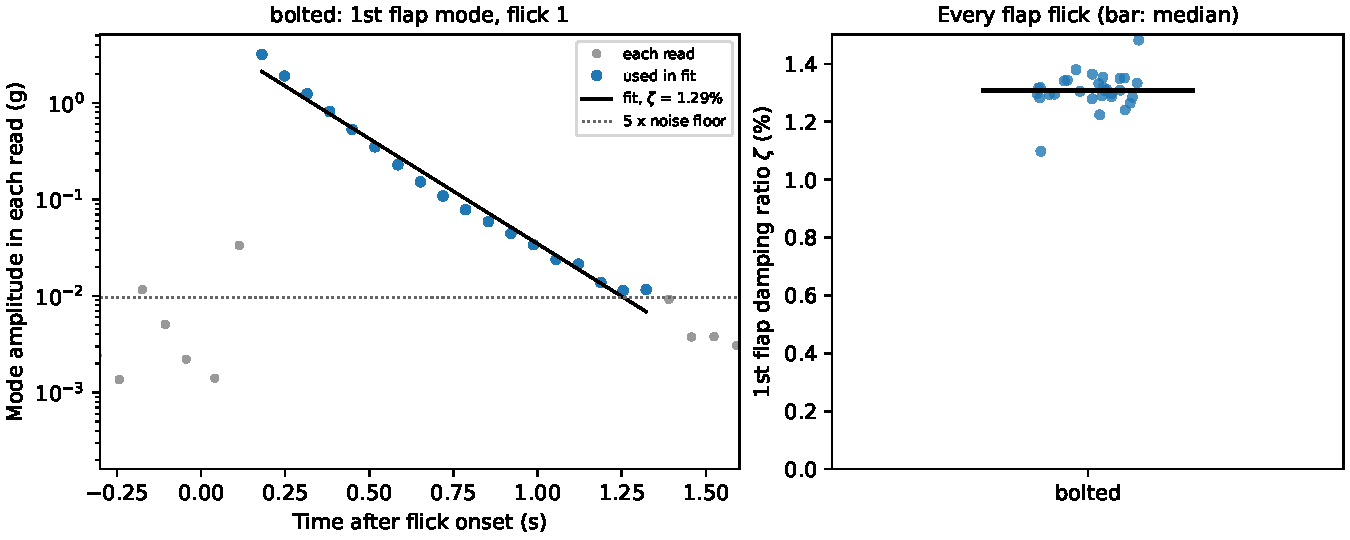
\includegraphics[width=0.9\textwidth]{figs/damping_bolted.pdf}
  \caption{Bolted blade, 62\,Hz peak, sensor~4 flapwise. Left: amplitude in
  each read after one flick, and the exponential fit; grey points are not
  used (before the peak or below five times the noise floor). Right: damping
  ratio of every flap flick.}
  \label{fig:damping_bolted}
\end{figure}

The 62\,Hz peak has a damping ratio of 1.31\% (median of 30 flicks, IQR
1.29--1.34\%). Each fit uses a median of 16 reads, spanning 0.2 to 1.2\,s
after the flick, as the amplitude falls from about 2\,g to 0.01\,g; the median
fit $R^2$ is 0.99. The flicks agree closely (Figure~\ref{fig:damping_bolted},
right).

\paragraph{The damping depends on amplitude.} The decay falls faster at large
amplitude than at small (the first points in Figure~\ref{fig:damping_bolted}
sit above the line). Fitting the first and second half of each decay
separately gives 1.57 and 1.06\%, so 1.31\% is an average over the amplitude
range of the fit.

\paragraph{Edgewise peaks: not measured reliably.} The damping script fits
the strongest edgewise peak, at 117\,Hz. The edgewise flicks die away within
about 0.3\,s, so only 14 of 30 flicks stay above five times the noise long
enough for a fit, each on the minimum of five reads. Their value
($\sim$2.3\%) is in the output files but should not be quoted. The 146\,Hz
peak has not been fitted. A measurement would need firmer edgewise flicks, or
captures without lost samples.

\section{Interpreting the bolted peaks with the beam model}
\label{sec:interp}

We first read the 117\,Hz peak as the first edge mode, since it is the
strongest edgewise peak in the edge flicks. The BeamDyn model of the blade
(\code{prototype-blade-exawind}, \code{docs/beam\_model/report.pdf},
3 November 2026) does not support that reading. The model clamps the blade
at the flange face and uses the datasheet modulus of Rigid~4000
($E = 4.1$\,GPa). It gives the first flap mode at 55.6\,Hz, the first edge
mode at 144.7\,Hz and the second flap mode at 165.0\,Hz. That report compared
the model with the earlier reading of this note (117\,Hz as the first edge
mode) and found that no single modulus fits; it listed the mode
identification as one possible cause.

\paragraph{Compare ratios, not frequencies.} The model is not calibrated: at
the datasheet modulus it is 11.5\% below the measured first flap mode, so
agreement in absolute frequency means little. Changing $E$ scales every
frequency by the same factor and leaves the ratios between modes unchanged,
so the ratios are the fair test (Table~\ref{tab:interp}).

\begin{table}[H]
  \centering
  \begin{tabular}{lccc}
    \toprule
    & Beam model & \multicolumn{2}{c}{Bolted ring-down} \\
    & & edge = 146\,Hz & edge = 117\,Hz \\
    \midrule
    1st flap (Hz) & 55.6 & 62 & 62 \\
    1st edge (Hz) & 144.7 & 146 & 117 \\
    2nd flap (Hz) & 165.0 & 162 & 162 \\
    \midrule
    1st edge / 1st flap & 2.60 & 2.35 ($-10\%$) & 1.89 ($-27\%$) \\
    2nd flap / 1st flap & 2.97 & 2.61 ($-12\%$) & 2.61 ($-12\%$) \\
    \bottomrule
  \end{tabular}
  \caption{Bolted ring-down against the clamped beam model, under either
  choice of first edge mode. Percentages: measured ratio against the model's.
  With $E$ raised to 5.1\,GPa to match the first flap mode, the model gives
  161\,Hz for the first edge and 184\,Hz for the second flap mode.}
  \label{tab:interp}
\end{table}

\paragraph{The first edge mode is at 146\,Hz.} Taking 146\,Hz as the first
edge mode, both of the model's ratios are about 10\% above the measured ones
(2.35 against 2.60, and 2.61 against 2.97). One cause acting on every mode
beyond the first could do that: the accelerometers and cables, which the
model leaves out, or a root that is slightly less than a clamp. Taking 117\,Hz
instead leaves the edge ratio 27\% low while the flap ratio is 12\% low, a
mismatch that would need a second, edge-only cause. The 146\,Hz peak also
behaves like a blade mode: it barely moves the root sensor
(Figure~\ref{fig:root}), as the flap modes do and as a clamped beam
predicts. It is rung flapwise by flap flicks too, which fits the flap--edge
coupling expected on a swept, twisted blade.

\paragraph{The 117\,Hz peak is most likely a mount mode.} The clamped model
has no mode between 55.6 and 144.7\,Hz, so the 117\,Hz peak is not a mode of
the blade as modelled. The data point to the mount, or the joint between
blade and mount:
\begin{itemize}
  \item It is the only edgewise peak at the root sensor, where the blade
        modes do not register (Section~\ref{sec:bolted}).
  \item The root moves with it, and in $z$ the three inner sensors move
        almost together: the whole blade moving on a compliant support, not
        the blade bending.
  \item It is the peak the bolt changes most (Section~\ref{sec:nobolt}).
  \item The mount is likely softest in this direction. The blade hangs from
        a solid metal arm (steel or aluminium) that points out sideways from
        a vertical shaft, with the blade's edgewise direction perpendicular to
        the shaft. The shaft is held by a servo motor. Edgewise motion at the
        root acts to turn the shaft. A solid metal arm and shaft are stiff
        next to a 23.5\,g blade, so the softest link is probably the servo:
        it resists rotation through its position control loop, gearing and
        coupling, which act as a torsional spring much softer than a clamp.
        Bending of the arm, especially if it is aluminium, may add to it. The whole blade swinging on that spring gives a
        low edgewise mode with the root moving, which a clamped beam model
        cannot contain.
\end{itemize}
This is a strong indication, not a proof: four sensors sample the span only
coarsely, and a mode that combines root rotation with blade bending could
look the same. An accelerometer on the mount during a ring-down, or root
springs in the beam model (already planned there for the no-bolt case),
would settle it: a mount mode near 117\,Hz should appear while the blade
modes stay close to their clamped values.

\paragraph{Mode labels used from here on.} 62\,Hz first flap, 117\,Hz mount
(likely), 146\,Hz first edge, 162\,Hz second flap. The higher peaks are
labelled by axis only (edgewise $\sim$300\,Hz, flapwise $\sim$400\,Hz,
edgewise $\sim$550\,Hz); the beam model report has not yet paired them with
model modes.

\section{With and without the bolt}
\label{sec:nobolt}

\subsection{Modes}

\begin{figure}[H]
  \centering
  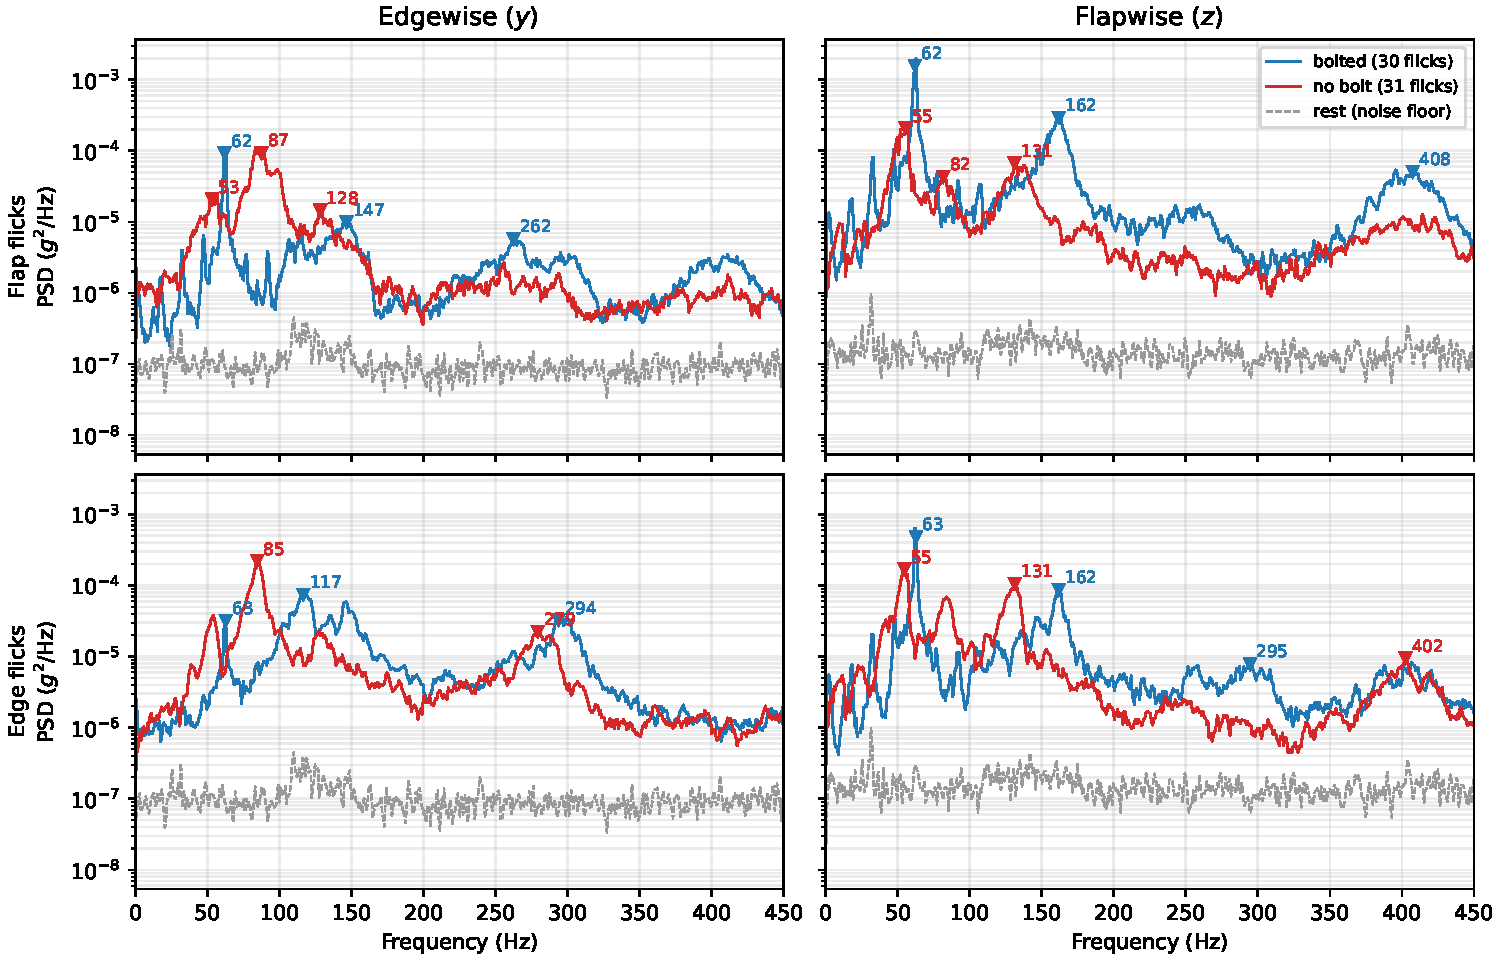
\includegraphics[width=\textwidth]{figs/ringdown_compare.pdf}
  \caption{As Figure~\ref{fig:bolted}, with the no-bolt run (red) added to
  the bolted one (blue).}
  \label{fig:compare}
\end{figure}

\begin{table}[H]
  \centering
  \begin{tabular}{lcccl}
    \toprule
    Mode & Bolted (Hz) & No bolt (Hz) & Change & Main axis \\
    \midrule
    1st flap  & 62  & 55  & $-11\%$ & $z$ \\
    mount (likely) & 117 & 85  & $-27\%$ & $y$ \\
    1st edge, 2nd flap & 146, 162 & 131, 138 & $-10$ to $-19\%$ & $z$ and $y$ \\
    edge, $\sim$300\,Hz & 294 & 279 & $-5\%$  & $y$ \\
    flap, $\sim$400\,Hz & 408 & 401 & $-2\%$ & $z$ \\
    edge, $\sim$550\,Hz & 536 & 555 & $+4\%$ & $y$ \\
    \bottomrule
  \end{tabular}
  \caption{Sensor~4 peaks with and without the bolt. Without the bolt the
  first edge and second flap modes become a pair at 131 and 138\,Hz that
  cannot be assigned one to one. The no-bolt run also has a weak peak at
  361\,Hz, and the bolted 259\,Hz peak has no clear partner. The three
  highest are uncertain by about 15\,Hz.}
  \label{tab:modes}
\end{table}

\paragraph{The bolt matters most for the low peaks.} The low peaks drop by
10--27\%; the higher ones by 5\% or less, within the uncertainty of those
peaks (Figure~\ref{fig:compare}, Table~\ref{tab:modes}). This is what a
softer root joint would do: the low modes swing the whole blade about its
root, while the higher modes bend the blade itself. The mount peak is the
most affected, from 117 to 85\,Hz. Without the bolt it is still the largest
peak at the root sensor, at 176 times the noise floor in $y$ and 158 times
in $z$.

\begin{figure}[H]
  \centering
  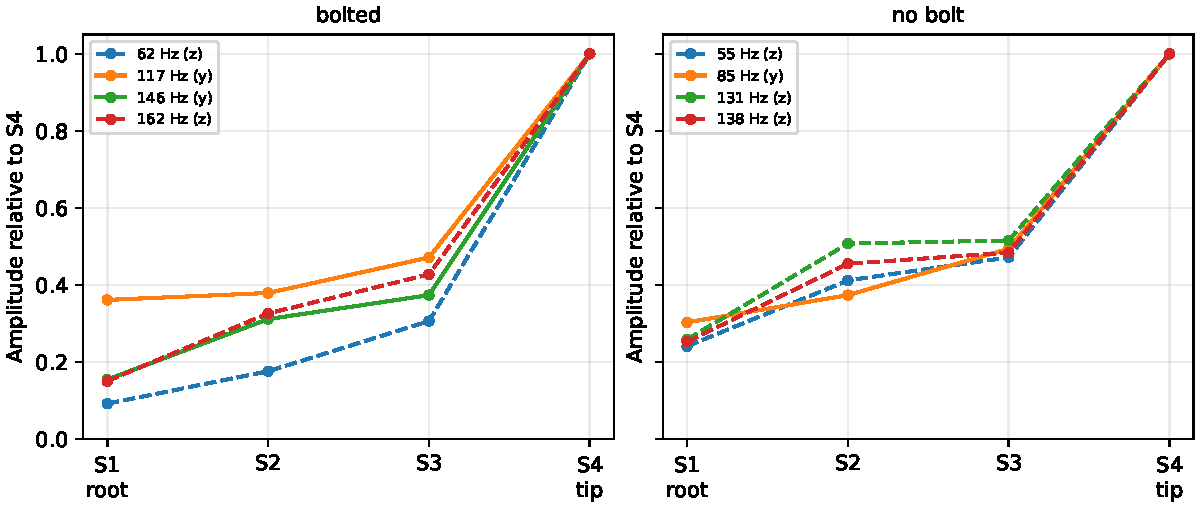
\includegraphics[width=0.8\textwidth]{figs/span_compare.pdf}
  \caption{Amplitude of each low peak along the span, relative to the tip,
  with and without the bolt (as Figure~\ref{fig:root}, right).}
  \label{fig:span}
\end{figure}

\paragraph{Without the bolt the root moves in every mode.} With the bolt,
only the 117\,Hz peak moves the root sensor much (36\% of the tip). Without
it, every low peak moves the root by about a quarter of the tip motion
(Figure~\ref{fig:span}). That is what a loose joint should do, but it also
means the span shape no longer singles out the mount peak the way it does
with the bolt.

\paragraph{The 146 and 162\,Hz modes become a close pair.} Without the bolt
there is no peak near 146 or 162\,Hz. Instead the flap flicks show two
peaks of almost the same height at 131 and 138\,Hz in $z$, and their span
shapes are the same. They are most likely the first edge and second flap
modes, moved down by 10--19\%, but these data cannot tell which is which.
As with the bolt, the flicks are not pure: here a flap flick rings the
85\,Hz peak in $y$ about half as strongly as the first flap mode in $z$.

\subsection{Damping}

\begin{figure}[H]
  \centering
  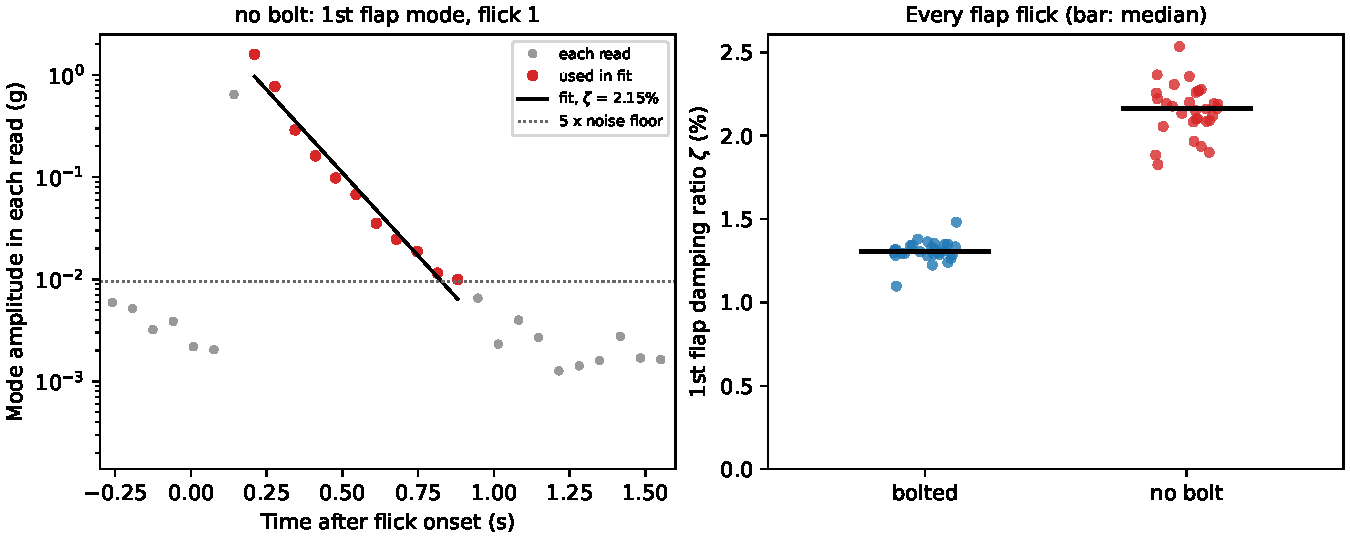
\includegraphics[width=0.9\textwidth]{figs/damping_compare.pdf}
  \caption{As Figure~\ref{fig:damping_bolted}. Left: one no-bolt flap flick.
  Right: every flap flick, with and without the bolt.}
  \label{fig:damping_compare}
\end{figure}

\begin{table}[H]
  \centering
  \begin{tabular}{lccccc}
    \toprule
    & Frequency & $\zeta$, median & IQR & Flicks & Reads per fit \\
    \midrule
    With the bolt    & 62.0\,Hz & 1.31\% & 1.29--1.34\% & 30 of 30 & 16 \\
    Without the bolt & 55.4\,Hz & 2.16\% & 2.09--2.26\% & 31 of 31 & 10 \\
    \bottomrule
  \end{tabular}
  \caption{Damping ratio of the first flap mode. Fits span 0.2 to 1.2\,s
  (bolted) and 0.2 to 0.8\,s (no bolt) after the flick, from about 2\,g down
  to 0.01\,g; median fit $R^2$ 0.99 and 0.97.}
  \label{tab:damping}
\end{table}

\paragraph{Without the bolt the first flap mode is damped about 65\% more}
(2.16 against 1.31\%), and again the flicks agree closely
(Figure~\ref{fig:damping_compare}, right).

\paragraph{The amplitude dependence is stronger.} Fitting the first and
second half of each decay gives 3.07 and 1.62\% without the bolt, against
1.57 and 1.06\% with it. This would fit friction or slip in the loose joint,
but these data do not show the mechanism.

\paragraph{Edgewise peaks.} Only 5 of 30 no-bolt edge flicks could be fitted
at the 85\,Hz mount peak ($\sim$3.9\%), even fewer than with the bolt; as
there, the value should not be quoted.

\section{Which configuration the experiments had}
\label{sec:production}

\begin{figure}[h]
  \centering
  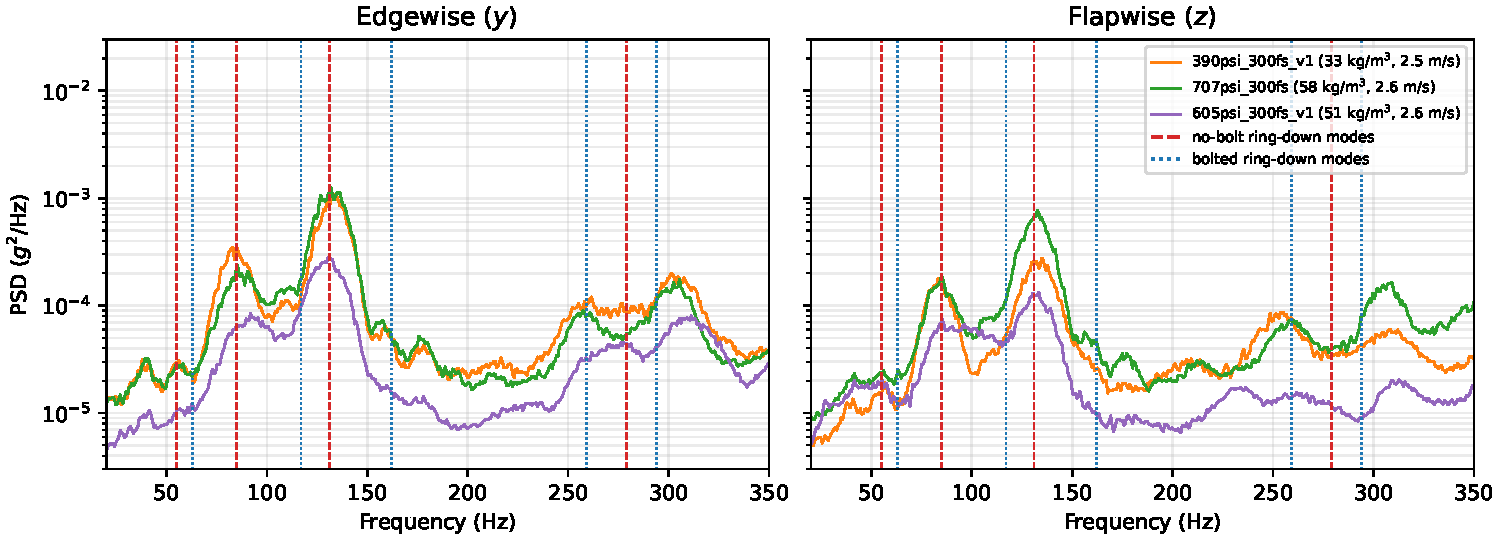
\includegraphics[width=\textwidth]{figs/production_slow.pdf}
  \caption{Sensor~4 PSD of the three slowest production runs (2.5--2.6\,m/s),
  median over the third of each run's angles with the least vibration, so the
  flow only nudges the blade. Dashed red: no-bolt modes; dotted blue: bolted
  modes.}
  \label{fig:production}
\end{figure}

In the experiments the flow excites the blade continuously. At low speed and
at the angles where the blade is quiet, that excitation is gentle and the
spectrum shows the blade's own frequencies, much as a ring-down does.
Figure~\ref{fig:production} shows these spectra for the three slowest runs,
at 33, 51 and 58\,kg/m$^3$, recorded on 6, 14 and 9 October.

All three peak at 84--86\,Hz and 131--133\,Hz in both axes: the no-bolt
mount peak and the 131/138\,Hz pair. None shows a peak at the bolted 117,
146 or 162\,Hz.
Since the slow runs span the campaign, the bolt was most likely missing
throughout, not lost partway. The order of the two ring-downs fits this: the
no-bolt run was recorded first, and the bolted one an hour later.

If the 85\,Hz peak is the loose mount, the largest low-speed response in the
experiments is the blade rocking on its mount, not a blade mode. That
matters for how the experimental spectra are read, and it is a reason to fit
the bolt in future runs.

One difference stands out. In the ring-down, the 131\,Hz peak is four to
five times stronger in $z$ than in $y$. In these runs it is about two to four
times stronger in $y$. So in the tunnel this peak moves mostly edgewise. With
two modes 7\,Hz apart in the ring-down, one being the first edge mode, the
flow may simply excite the edgewise one of the pair more; the pressurized gas
changing the mode shapes would also do it. Plots of the experiments should
mark it by frequency (131\,Hz), not as a flapwise or edgewise mode.

The peaks near 300\,Hz in Figure~\ref{fig:production} (301--310\,Hz) sit
between the no-bolt (279\,Hz) and bolted (294\,Hz) second edge mode, within
the uncertainty of that frequency, so they do not tell the two apart.

\paragraph{At high speed the ring-down frequencies no longer describe the
blade.} Figure~\ref{fig:fast} repeats Figure~\ref{fig:production} for the
fastest run at each of the same three pressures. Even at the quietest angles
the spectrum is now about ten times higher, and the 85 and 131\,Hz peaks
have all but gone. At 6.9\,m/s both axes show a single peak at
109--111\,Hz, which matches neither no-bolt mode: the PSD there is about ten
times that at 85\,Hz and three times that at 131\,Hz. The 6.0\,m/s run sits
in between, with two peaks (95--96 and 122--125\,Hz), each pulled from a
no-bolt mode toward 110\,Hz. The 110\,Hz peak is also 6--7\% below the
bolted first edge mode (117\,Hz), so it is not the bolted blade either.

So the ring-down modes describe the blade at low speed only. At speed the
flow changes the frequencies the blade responds at, and the experiments
cannot be read against the ring-down frequencies alone. One explanation
consistent with Figure~\ref{fig:fast} is that the flow couples the 85 and
131\,Hz modes and draws them together as the speed rises; the three runs
here are not enough to show it.

\begin{figure}[h]
  \centering
  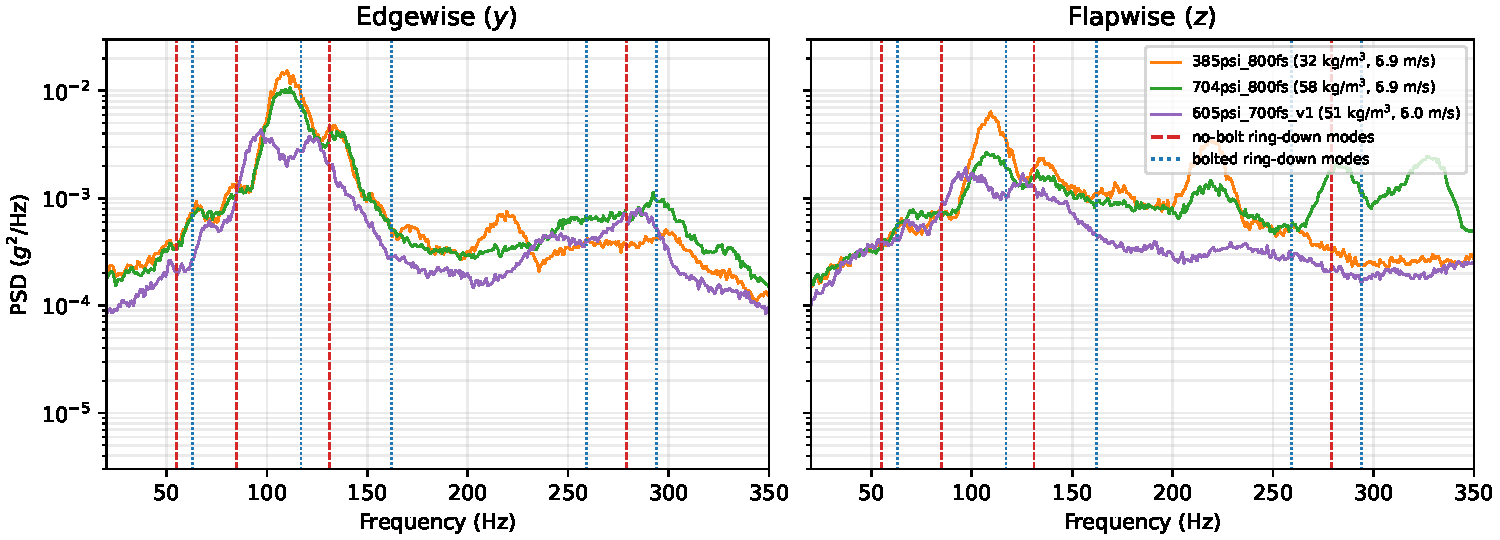
\includegraphics[width=\textwidth]{figs/production_fast.pdf}
  \caption{As Figure~\ref{fig:production}, for the fastest run at each
  pressure (6.0--6.9\,m/s; 605\,psi went only to 6.0\,m/s), on the same
  scale.}
  \label{fig:fast}
\end{figure}

\section{Caveats}

\begin{itemize}
  \item We assume both ring-downs were done at atmospheric pressure, with the
        tunnel not pressurized. The experiments ran in gas 27--95 times
        denser. A rough flat-plate estimate puts the effect of the heavier gas
        on the flap modes at a few percent (more at 1414\,psi) and on the
        edge modes at under 1\%, but this has not been measured.
  \item The flicks were by hand, so their direction and strength vary. The
        median over 30 flicks takes care of the strength, not the direction.
  \item Sensor~4 is used for the frequencies; the other sensors give the same
        low-mode frequencies. All four are used only for the span shapes in
        Figures~\ref{fig:root} and~\ref{fig:span}, which ignore the sensors'
        exact positions.
  \item Calling 117\,Hz (85\,Hz without the bolt) a mount mode rests on the
        root sensor and the span shape, not on a measurement of the mount.
  \item The sample rate (1493\,Hz) comes from the vendor's measurement, not
        from our data. The low modes do not depend on it; the modes above
        150\,Hz move by up to 15\,Hz with it.
\end{itemize}

\section{Recommendations}

\begin{enumerate}
  \item \textbf{Use the no-bolt frequencies for the production runs} once the
        mount state is confirmed. \code{plot\_psd.py} holds them
        (\code{NATURAL\_HZ}: 55, 85, 131, 279 and 401\,Hz; 138\,Hz should be
        added, and 85\,Hz labelled as the mount); the current production
        figures leave them out (\code{--no-modes}) until then.
  \item \textbf{Confirm the mount mode.} Put an accelerometer on the mount
        (or tap the mount itself) during a bolted ring-down: a mount mode
        shows up strongly there at 117\,Hz. If the servo is the soft link,
        repeating a few flicks with the drive disabled, or with different
        servo gains, should move the 117\,Hz peak while the 62, 146 and
        162\,Hz modes stay put. Record the servo state (enabled, gains) in
        \code{run\_metadata.json} for every ring-down and production run. Alternatively, add a rotational
        spring at the root of the beam model and see whether a low edgewise
        mode near 117\,Hz appears while 62, 144 and 162\,Hz stay put.
  \item \textbf{Record the mount state in \code{run\_metadata.json}} (bolt
        fitted, torque), and check it at the start of each test day.
  \item \textbf{Repeat the no-bolt ring-down in the pressurized tunnel with
        the fans off,} at one low and one high pressure (e.g.\ 385 and
        1414\,psi). Any shift from 85, 131 and 138\,Hz is then the effect of the
        gas alone.
  \item \textbf{Decide whether future runs use the bolt.} The two
        configurations give different natural frequencies, so runs with and
        without it should not be mixed.
\end{enumerate}

\paragraph{Reproducing.} \code{python3 reports/ringdown/make\_figures.py}
from the repository root writes all figures and prints every number quoted
here, including the damping fits and the synthetic check. It needs the two ring-down folders in \code{data/} and the production
summaries from \code{extract\_run\_summary.py}~1.4.

\end{document}
